\chapter{Master flat y calibración final}
\setcounter{ipythcntr}{0}

En las clases anteriores aprendimos a crear archivos master bias y master dark. Lo único que queda por hacer es crear un archivo master flat con las imágenes de flat fields y así podremos finalmente realizar la calibración básica de nuestros datos. Esta tarea también se consigue utilizando el paquete \pynorm{ccdproc}. También utilizaremos unas cuantas funciones de \pynorm{astropy} y \pynorm{numpy}, así como las herramientas de visualización de Python.  

\section{Calibración de imágenes}
Ahora trabajaremos con las imágenes de flat fields, con las que vamos a necesitar realizar un poco más de tareas, pero nada muy complicado. Recuerda que este documento es solo un resumen de los pasos necesarios para realizar la calibración, para más detalles de los pasos y los códigos, debes revisar el Notebook llamado \norbash{Example-FLAT.ipynb}. 

\subsection{Creando un archivo master flat}
Volveremos a utilizar el módulo \pynorm{ccdproc} junto con sus submódulos y funciones. Por lo tanto, como es usual, primero importamos todo lo que usaremos en nuestro código:

\begin{pyin}[]
#- Para trabajar con rutas
from pathlib import Path

#- Modulos de astropy y ccd proc
from astropy import units as u
from astropy.nddata import CCDData
from ccdproc import ImageFileCollection
from  ccdproc import substract_overscan, trim_image, substract_dark

#- Módulos para estadística
import numpy as np
from astropy.stats import mad_std

#- Modulos para visualización
from show_image import show_image 
\end{pyin}

Como encontramos anteriormente, las imágenes de corriente oscura tienen diferentes tiempos de exposición. Las imágenes de flat también tienen diferentes tiempos de exposición. Para poder corregir las imágenes flat por corriente oscura, necesitamos agruparlas de acuerdo al tiempo de exposición para que coincidan con las de corriente oscura. La función que nos ayudará a conseguirlo se llama \pynorm{find_nearest_dark_exposure()} y debemos importarla.

\begin{pyin}
from functions import find_nearest_dark_exposure
\end{pyin}

Ya que hemos definido los módulos a utilizar, podemos ahora definir las variables que nos darán acceso a los archivos:
\begin{pyin}[]
#- Definiendo la ruta a los datos
cryo_path = pathlib.Path('example-cryo-LFC')
calibrated_data = Path('example-reduced')

#- Selecciona las imágenes
files = ImageFileCollection(cryo_path)
reduced_images = ImageFileCollection(calibrated_data)
combined_dark_files = reduced_images.files_filtered(imagetyp='dark', 
                                                    combined=True)
\end{pyin}

Al igual que con las imágenes de bias y corriente oscura, necesitaremos restar el overscan y recortar las imágenes flat. Adicionalmente, también debemos corregir por corriente oscura. Primero veamos cómo hacerlo para una sola imagen y luego lo aplicaremos a todas. Seleccionamos una sola imagen flat:
\begin{pyin}[]
#- Seleccionando una imagen flat
a_flat = CCDData.read(files.files_filtered(imagetyp='flatfield',
                    include_path=True)[0], unit='adu')
\end{pyin}

Y ahora podemos corregirla por overscan y recortarla:
\begin{pyin}[]
# Restar el overscan
a_flat_reduced = subtract_overscan(a_flat, 
                                        overscan=a_flat[:, 2055:], 
                                        median=True)

# Recortar
a_flat_reduced = trim_image(a_flat_reduced[:, :2048])

# Visualizar
show_image(a_flat_reduced, cmap='gray')
plt.title('Single flat frame, overscan subtracted and trimmed')
\end{pyin}

En la Figura \ref{fig:flat_comparison} se muestra una comparación entre la imagen flat sin procesar y luego de ser procesada. 

\begin{figure}[htb]
  \centering
	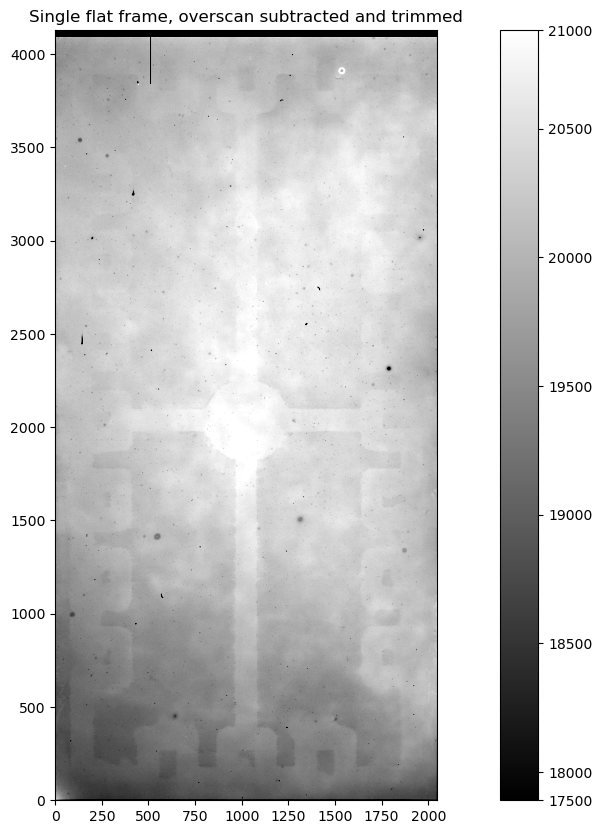
\includegraphics[width=0.45\textwidth]{figures/flat_trimmed.png}
	\caption{Una imagen flat antes y después de restar el overscan y recortarla}
	\label{fig:flat_comparison} 
\end{figure}

Revisamos los tiempos de exposición para las imágenes flat:

\begin{pyin}
set(files.summary['exptime'][files.summary['imagetyp'] == 'FLATFIELD'])
\end{pyin}
\begin{pyprint}
{7.0, 70.001, 70.011}
\end{pyprint}

Y comparamos con los de corriente oscura:
\begin{pyin}
actual_exposure_times = set(h['exptime'] for h in reduced_images.headers(imagetyp='dark', combined=True))
actual_exposure_times
\end{pyin}
\begin{pyprint}
{7.0, 70.0, 300.0}
\end{pyprint}

Comprobamos a cuál de estos tiempos de exposición está más cercano el de la imagen flat con ayuda de la función \pynorm{find_nearest_dark_exposure}:

\begin{pyin}
closest_dark = find_nearest_dark_exposure(a_flat_reduced, actual_exposure_times)
closest_dark
\end{pyin}
\begin{pyout}
70.0
\end{pyout}

Ahora creamos un diccionario con las tres imágenes master dark que generamos anteriormente:

\begin{pyin}
combined_darks = {ccd.header['exptime']: ccd for ccd in reduced_images.ccds(imagetyp='dark', combined=True)}
\end{pyin}

Y ahora restamos el master dark correspondiente a los $ 70 \mathrm{~s} $ de exposición a la imagen flat que seleccionamos:

\begin{pyin}
a_flat_reduced = subtract_dark(a_flat_reduced, 
                               combined_darks[closest_dark], 
                               exposure_time='exptime', 
                               exposure_unit=u.second, scale=False)
\end{pyin}

Este último archivo está corregido por overscan, está recortado y además está corregido por corriente oscura. Ahora podemos aplicar este procedimiento a todas las imágenes flat en un bucle \pynorm{for} de la siguiente manera:

\begin{pyin}
for ccd, file_name in files.ccds(imagetyp='FLATFIELD',
                                 ccd_kwargs={'unit': 'adu'},
                                 return_fname=True):    
    # Subtract the overscan
    ccd = subtract_overscan(ccd, overscan=ccd[:,2055:], median=True)
    
    # Trim the overscan
    ccd = ccdp.trim_image(ccd[:, :2048])
    
    # Find the correct dark exposure
    closest_dark = find_nearest_dark_exposure(ccd, 
                                              actual_exposure_times)
    
    # Subtract the dark current 
    ccd = subtract_dark(ccd, combined_darks[closest_dark],
                        exposure_time='exptime', 
                        exposure_unit=u.second)

    # Save the result; 
    ccd.write(calibrated_data / ('flat-' + file_name))
\end{pyin}
 
 Antes de combinar los flats, debemos actualizar la carpeta de imágenes calibradas y separarlas por sus filtros. En este conjunto de datos en particular, se utilizaron los filtros i y g:
 
\begin{pyin}[]
#- Actualizando el contenido de la carpeta
reduced_images.refresh()

#- Definiendo el tipo de imagen
flat_imagetyp = 'flatfield'

#- Buscando los filtros usados en este tipo de imagen
flat_filters = set(h['filter'] for h in
                   reduced_images.headers(imagetyp=flat_imagetyp))
flat_filters
\end{pyin}
\begin{pyprint}
{"g'", "i'"}
\end{pyprint}

Vamos a definir una función que nos ayudará a mejorar la estadística al momento de combinar los flats.

\begin{pyin}
def inv_median(a):
    return 1 / np.median(a)
\end{pyin}

Ahora creamos el master flat para cada filtro:

\begin{pyin}
for filt in flat_filters:
    to_combine = reduced_images.files_filtered(
                                imagetyp=flat_imagetyp, 
                                filter=filt, include_path=True)
                                
    combined_flat = ccdp.combine(to_combine,
                                 method='average', 
                                 scale=inv_median,
                                 sigma_clip=True, 
                                 sigma_clip_low_thresh=5, 
                                 sigma_clip_high_thresh=5,
                                 sigma_clip_func=np.ma.median,
                                 signma_clip_dev_func=mad_std,
                                 mem_limit=350e6
                                )

    combined_flat.meta['combined'] = True
    
    flat_file_name = 'combined_flat_filter_{}.fits'.format(filt.replace("''", "p"))
    combined_flat.write(calibrated_data / flat_file_name)
\end{pyin}
 
 Actualizamos nuevamente la carpeta de imágenes calibradas:
 
 \begin{pyin}[]
#- Actualizando el contenido de la carpeta
reduced_images.refresh()
 \end{pyin}
 
 En la Figura \ref{fig:master_flats} se muestran las imágenes master flat para cada filtro:
 
 \begin{figure}[htb]
   \centering
	 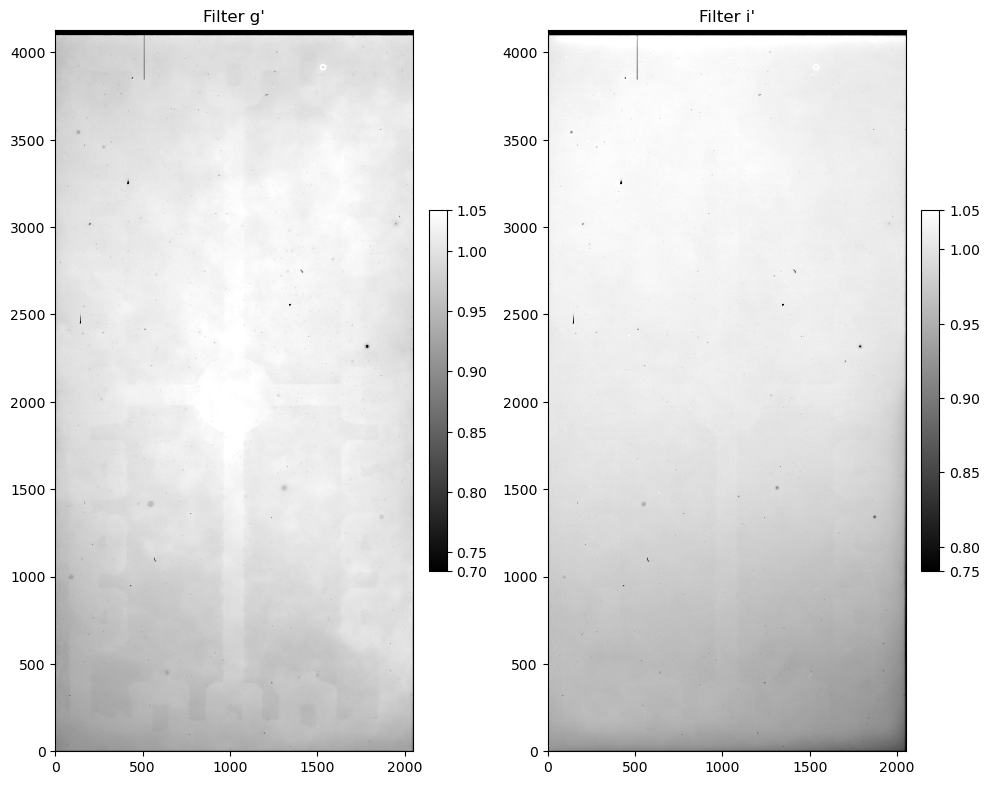
\includegraphics[width=0.8\textwidth]{figures/master_flats.png}
	 \caption{Archivos master flats para cada filtro.}
	 \label{fig:master_flats} 
 \end{figure}
 
 \subsection{Calibrando las imágenes de objeto}
En nuestra carpeta de imágenes sin procesar, solo hay dos imágenes de objeto. Una para el filtro g y otra para el filtro i. Estas dos imágenes son a las que les aplicaremos las correcciones con los archivos master bias, master dark y master flat que ya hemos creado. Primero definimos un par de variables:

\begin{pyin}[]
#- Definiendo algunas variables
science_imagetyp = 'object'
exposure = 'exptime'
\end{pyin} 

Definimos un diccionario con los master flat:
\begin{pyin}
combined_flats = {ccd.header['filter']: ccd for ccd in reduced_images.ccds(imagetyp=flat_imagetyp, combined=True)}
\end{pyin}

Y finalmente realizamos la calibración básica con un bucle \pynorm{for}:

\begin{pyin}[]
#- Definiendo listas vacías
all_reds = []
light_ccds = []

#- Ciclo for para reducir las imágenes
for light, file_name in files.ccds(imagetyp=science_imagetyp, return_fname=True, ccd_kwargs=dict(unit='adu')):

    #- Incluyendo un nuevo elemento a la lista
    light_ccds.append(light)
    
    #- Restando overscan de la image de objeto
    reduced = ccdp.subtract_overscan(light, overscan=light[:, 2055:], median=True)
    
    #- Cortando la imagen de objeto
    reduced = ccdp.trim_image(reduced[:, :2048])

    #- Decidiendo cuál tiempo de exposición usar
    closest_dark = find_nearest_dark_exposure(reduced, combined_darks.keys())

    #- Corrigiendo por corriente oscura
    reduced = ccdp.subtract_dark(reduced, combined_darks[closest_dark],
                                 exposure_time=exposure, exposure_unit=u.second)
    
    #- Seleccionando el flat adecuado de acuerdo al filtro
    good_flat = combined_flats[reduced.header['filter']]

    #- Corrigiendo por flat
    reduced = ccdp.flat_correct(reduced, good_flat)

    #- Incluyendo un nuevo elemento a la lista
    all_reds.append(reduced)

    reduced.write(calibrated_data / file_name)
\end{pyin}
 
 Los resultados de la calibración se muestran en la Figura \ref{fig:reduced_images}.
 
 \begin{figure}[htb]
   \centering
	 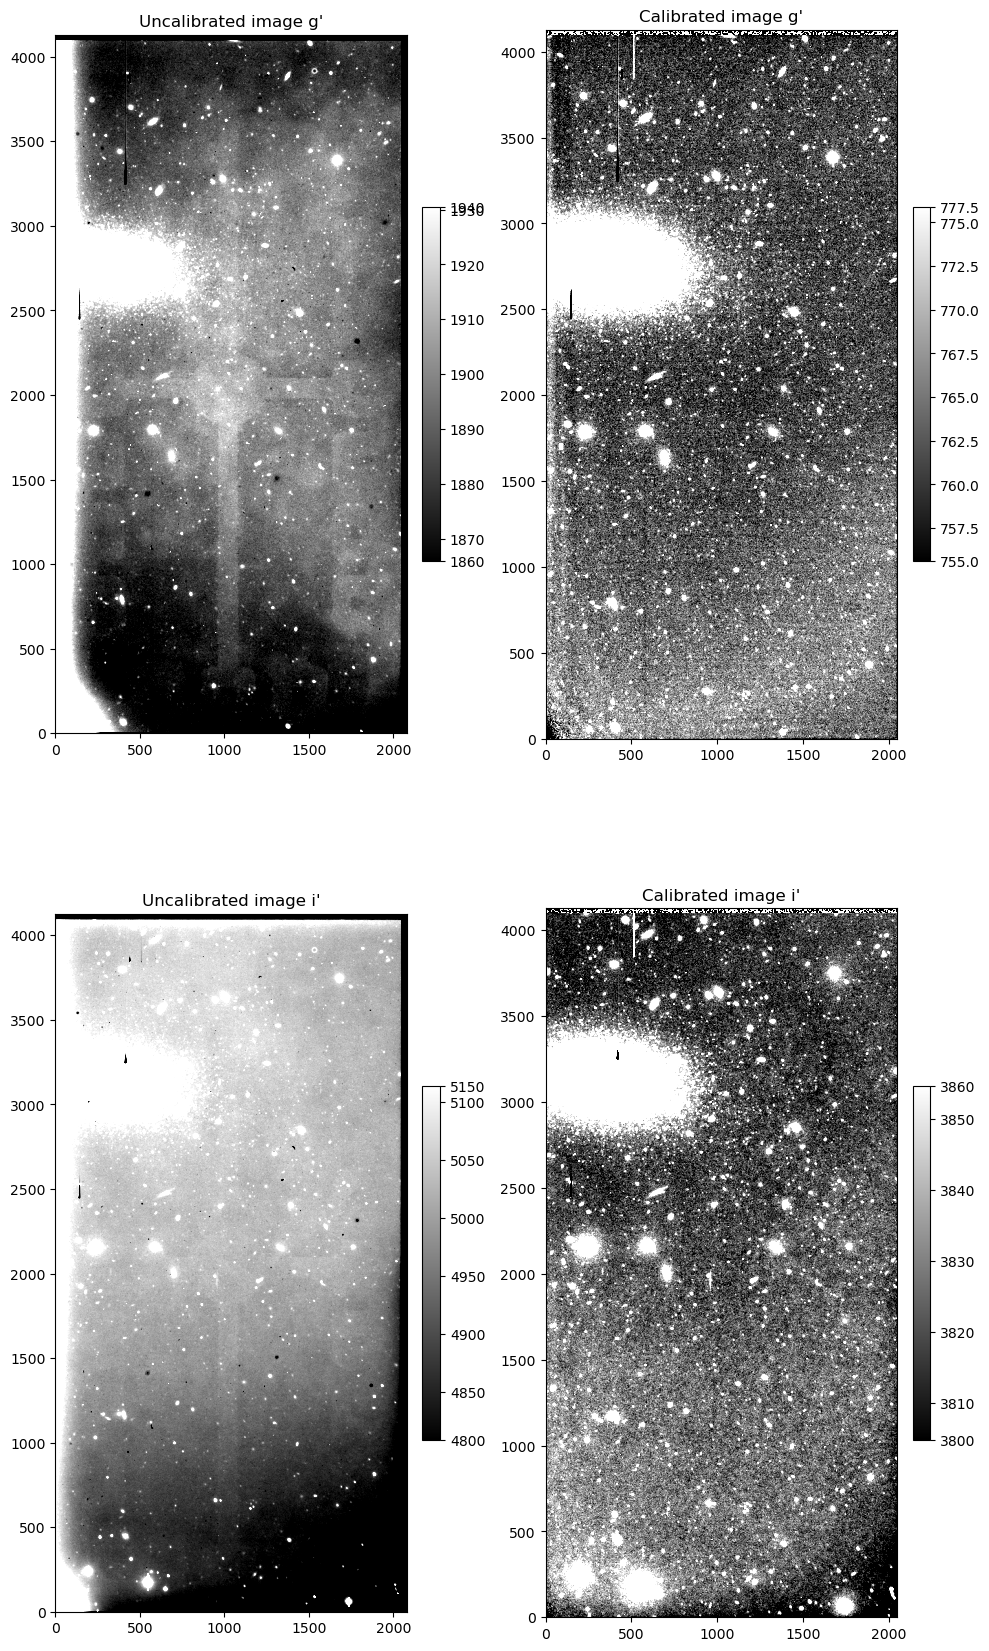
\includegraphics[width=0.8\textwidth]{figures/reduced_images.png}
	 \caption{Comparación de imágenes calibradas y no calibradas en diferentes filtros}
	 \label{fig:reduced_images} 
 \end{figure}
 
 
 
 
 
 
 
